\documentclass[aspectratio=169]{beamer}

%==============================================================================
% Aanloop
%==============================================================================

%---------- Packages ----------------------------------------------------------

\usepackage{etex}
\usepackage{graphicx,multicol}
\usepackage{comment,enumerate,hyperref}
\usepackage{amsmath,amsfonts,amssymb}
\usepackage{tikz}
\usepackage[dutch]{babel}
\usepackage{multirow}
\usepackage{eurosym}
\usepackage{listings}
\usepackage{textcomp}
\usepackage{framed}
\usepackage{wrapfig}
\usepackage{pgf-pie}
\usepackage{pgfplots}
\usepackage{booktabs}
\usepackage{pgfplotstable}
\usepackage{changepage}

%---------- Configuratie ------------------------------------------------------

\usetikzlibrary{arrows,shapes,backgrounds,positioning,shadows}
\usetikzlibrary{pgfplots.statistics}

\usetheme{hogent}
\usecolortheme{hgwhite} % witte achtergrond, zwarte tekst

%\setbeameroption{show notes}

%---------- Commando-definities -----------------------------------------------

\newcommand{\tabitem}{~~\llap{\textbullet}~~}
\renewcommand{\arraystretch}{1.2}

%---------- Info over de presentatie ------------------------------------------

\title[OZT: Analyse 2 variabelen]{Les 5. Analyse van 2 variabelen}
\subtitle{Onderzoekstechnieken}
\author{Jens Buysse \and Wim {De Bruyn} \and Bert {Van Vreckem}}
\date{AJ 2018-2019}

%==============================================================================
% Inhoud presentatie
%==============================================================================

\begin{document}

%---------- Front matter ------------------------------------------------------

\begin{frame}
\maketitle
\end{frame}

\begin{frame}
\frametitle{What's on the menu today?}

\tableofcontents
\end{frame}


%---------- Bivariate Analyse---------------------------------------------------
\section{Bivariate Analyse}
\begin{frame}
  \frametitle{Bivariate Analyse}
  \note{Deze slide wordt gebruikt om een voorbeeld te geven van een minder triviaal verband tussen variabelen: Ant Colony optimization. Verbanden tussen variabelen zouden dus kunnen zijn:

  \begin{itemize}
    \item Aantal obstakels tussen nest en voedeselbron
    \item Algoritme gebruikt om feromonen weg te nemen / te plaatsen
    \item Vorm van de obstakels tussen nest en voedselbron
    \item \dots
  \end{itemize}}
  \begin{figure}
    \centering
    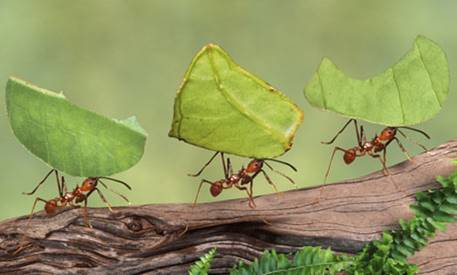
\includegraphics[width=0.8\textwidth]{img/ants.jpg}
    \label{fig:ants}
  \end{figure}

\end{frame}

\subsection{Bivariate Analyse: grafisch}

\begin{frame}
  \frametitle{Voorbeeld}
  \framesubtitle{Tevredenheidsonderzoek campusrestaurant}


  \begin{itemize}
    \item Hoe vaakt bezoekt men het restaurant?
    \item Is er een verschil in uitgaven tussen student en medewerker?
    \item Is er een verband tussen het aantal dagen dat men bezoekt en bedrag dat men wekelijks besteedt?
  \end{itemize}

  R Code: zie \texttt{cursus/data/catering\_hogeschool.R}

  \centering
  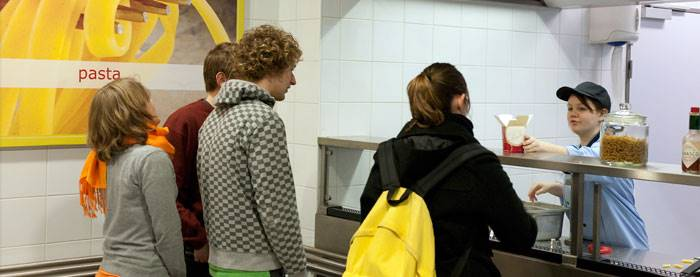
\includegraphics[height=.4\textheight]{img/students.jpg}
\end{frame}

\begin{frame}{Hoe vaakt bezoekt men het restaurant?}
  \begin{columns}
    \begin{column}{0.5\textwidth}
      \begin{table}[h]
        \small
        \begin{tabular}{|l|l|}
          \hline
          { \textbf{Statistiek}} & \textbf{Waarde} \\ \hline
          Mean                   & 2.96            \\ \hline
          Median                 & 3               \\ \hline
          Mode                   & 2               \\ \hline
          Stdev                  & 1.484           \\ \hline
          Variantie              & 2.202           \\ \hline
          Range                  & 4               \\ \hline
          $Q_{1}$                & 2               \\ \hline
          $Q_{2}$                & 3               \\ \hline
          $Q_{3}$                & 5               \\ \hline
        \end{tabular}
      \end{table}
    \end{column}
    \begin{column}{0.5\textwidth}

      \begin{figure}
        \centering
        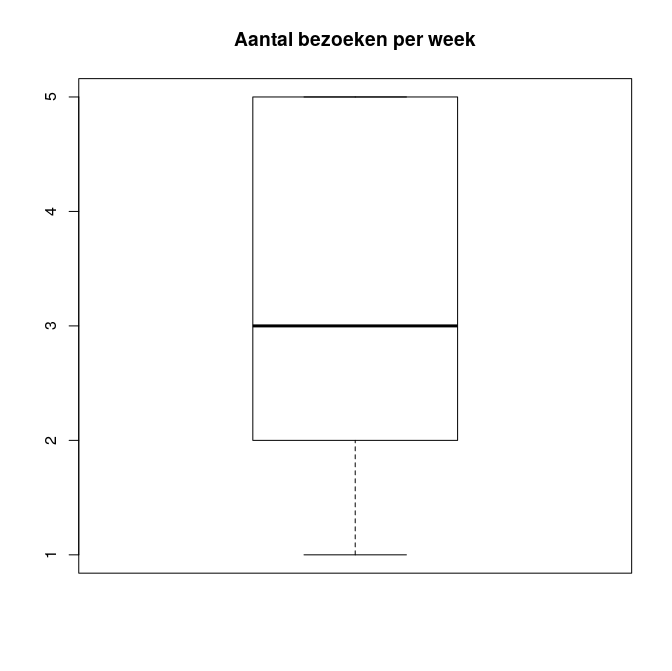
\includegraphics[height=.8\textheight]{img/2var-boxplot-aantalbezoeken}
        \label{fig:boxplotStudenten}
      \end{figure}

    \end{column}
  \end{columns}
\end{frame}

\begin{frame}{Hoe vaakt bezoekt men het restaurant?}
  
  \begin{columns}
    
    \begin{column}{0.5\textwidth}
      \begin{figure}
        \centering
        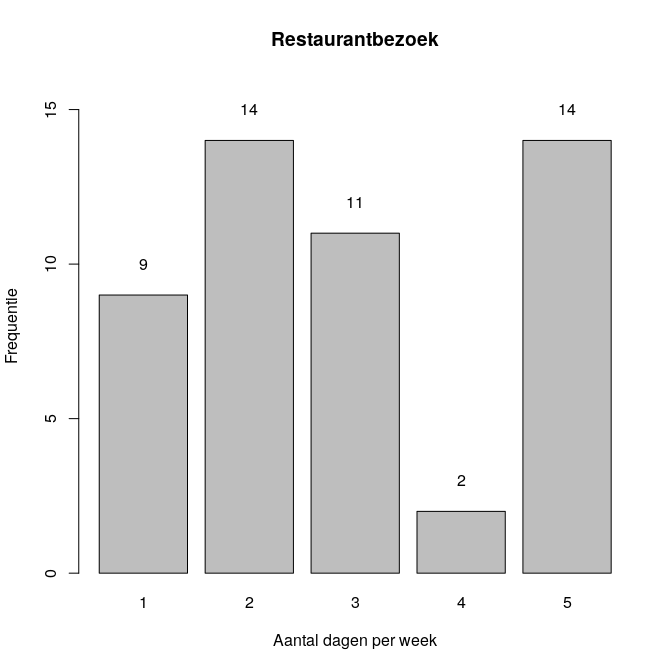
\includegraphics[height=.8\textheight]{img/2var-barplot-aantalbezoeken}
        \label{fig:studentenbar}
      \end{figure}
    \end{column}
  
    \begin{column}{0.5\textwidth}
      \begin{figure}
        \centering
        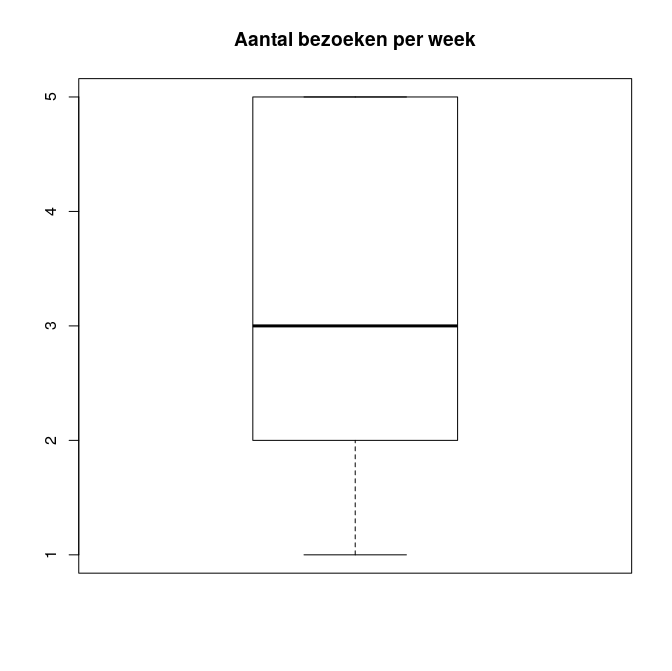
\includegraphics[height=.8\textheight]{img/2var-boxplot-aantalbezoeken}
        \label{fig:boxplotStudenten2}
      \end{figure}
    \end{column}
  
  \end{columns}
\end{frame}

\begin{frame}{Student vs werknemer}
  
  \begin{itemize}
    \item \alert<1>{Enkelvoudig staafdiagram} (van gemiddelde per categorie)
    \item \alert<2>{Boxplot}
  \end{itemize}

  \begin{figure}
    \centering
    \only<1>{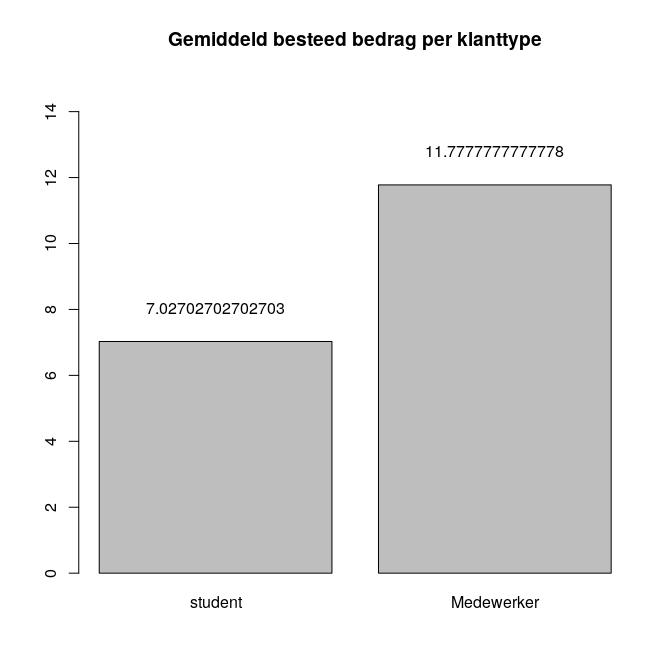
\includegraphics[height=0.6\textheight]{img/2var-barplot-gemiddeld-bedrag}}
    \only<2>{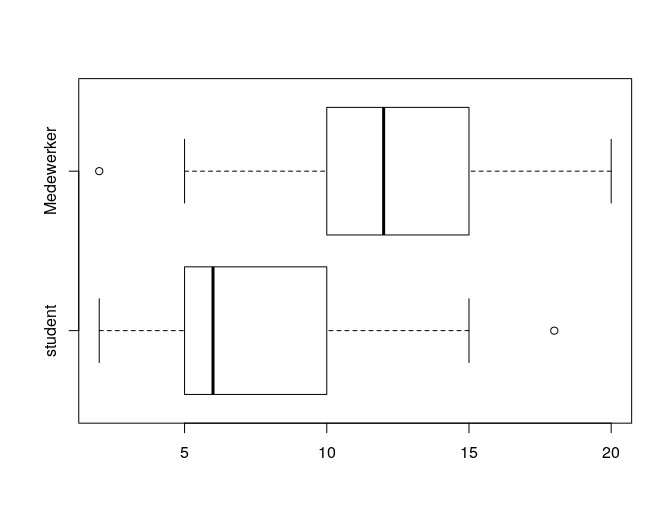
\includegraphics[height=0.6\textheight]{img/2var-boxplot-klanttype-bedrag}}
  \end{figure}

  \only<1>{\textbf{Let op!} Onvoldoende om significant verschil aan te tonen!}
\end{frame}

\begin{frame}
  \frametitle{Afhankelijke en onafhankelijke variabele}
  
  \begin{columns}
    \begin{column}{0.3\textwidth}

      \begin{figure}
        \centering
        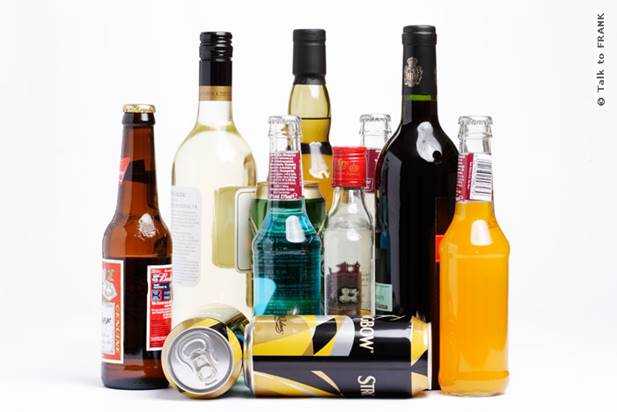
\includegraphics[width=1.00\textwidth]{img/liquor.jpg}
        \label{fig:liquor}
      \end{figure}

    \end{column}
    \begin{column}{0.3\textwidth}

      \begin{figure}
        \centering
        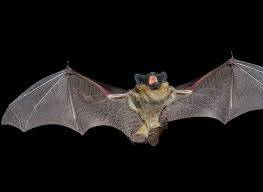
\includegraphics[width=1.00\textwidth]{img/bat.jpg}
        \label{fig:bat}
      \end{figure}

    \end{column}
    \begin{column}{0.3\textwidth}

      \begin{figure}
        \centering
        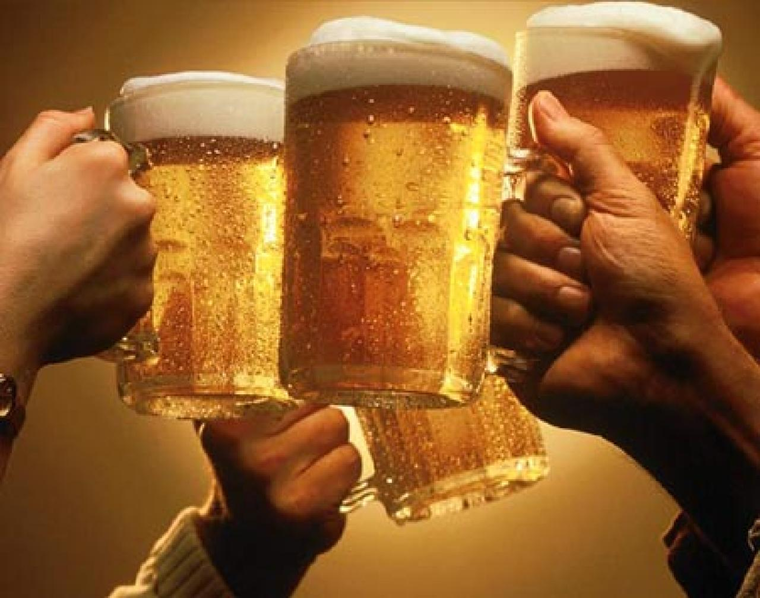
\includegraphics[width=1.00\textwidth]{img/beer.png}
        \label{fig:beer}
      \end{figure}

    \end{column}
  \end{columns}
  \note{Onderzoeken die hier gevoerd zijn:

  \begin{itemize}
    \item Invloed van alcoholinname op leervermogen van vleermuizen (Drinking and Flying: Does Alcohol Consumption Affect the Flight and Echolocation Performance of Phyllostomid Bats?)
    \item Arnd Leike of the Ludwig Maximilians University receives one of the Ig Nobel awards - which are given for research that cannot or should not be repeated - for demonstrating that beer froth obeys the mathematical law of exponential decay.
  \end{itemize}}
\end{frame}

\begin{frame}
  \frametitle{Onderzoek academiejaar 2013-2014}
  \begin{columns}
    \begin{column}{0.3\textwidth}

      \begin{figure}
        \centering
        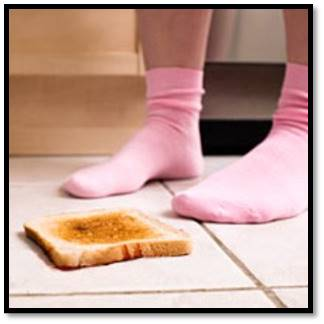
\includegraphics[width=1.00\textwidth]{img/toast.jpg}
        \label{fig:toast}
      \end{figure}

    \end{column}
    \begin{column}{0.3\textwidth}

      \begin{figure}
        \centering
        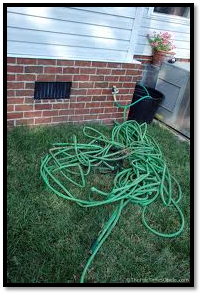
\includegraphics[width=1.00\textwidth]{img/hose.png}
        \label{fig:hose}
      \end{figure}

    \end{column}
    \begin{column}{0.3\textwidth}

      \begin{figure}
        \centering
        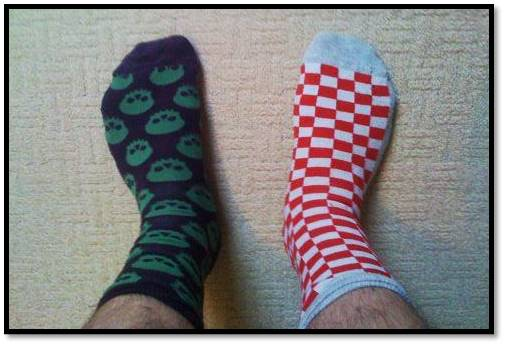
\includegraphics[width=1.00\textwidth]{img/socks.jpg}
        \label{fig:socks}
      \end{figure}

    \end{column}
  \end{columns}
  \note{Studenten moesten onderzoeken of er een verband was tussen vallen van boterham op boterzijde en hoogte e.a., of verband was tussen het aantal onpare sokken en andere fenomenen zoals je eigen was doen, veel sporten al dan niet \dots}
\end{frame}

\section{Kruistabellen en Cramér's V}

\begin{frame}
  \frametitle{Kruistabellen}
  Is er een verschil in waardering in het assortiment tussen mannen en vrouwen?

  \begin{table}[h]
    \begin{tabular}{l||l|l||l}
      & Vrouw & Man & Totaal \\ \hline \hline
      Goed        & 9     & 8   & 17     \\
      Voldoende   & 8     & 10  & 18     \\
      Onvoldoende & 5     & 5   & 10     \\
      Slecht      & 0     & 4   & 4      \\ \hline \hline
      Totaal      & 22    & 27  & 49     \\
    \end{tabular}
  \end{table}
\end{frame}

\begin{frame}
  \frametitle{Kruistabellen: percenteren}
  Is er een verschil in waardering in het assortiment tussen mannen en vrouwen?
  \begin{adjustwidth}{-1.5em}{-1.5em}
    \begin{table}[h] \centering
      \begin{tabular}{@{}rrrrrrr@{}} \toprule
        & Vrouw & Man & Totaal & Vrouw \% & Man\%   & Totaal  \\ \midrule
        Goed        & $9$     & $8$  & $17$     & $41$\%  & $30$\%  & $35$\% \\
        Voldoende   & $8$     & $10$ & $18$     & $36$\%  & $37$\%  & $37$\% \\
        Onvoldoende & $5$     & $5$  & $10$     & $23$\%  & $18$\%  & $20$\% \\
        Slecht      & $0$     & $4$  & $4$      & $0$\%   & $15$\%  & $8$\%  \\
        Totaal      & $22$    & $27$ & $49$     & $100$\% & $100$\% & $100$\%\\
        \bottomrule
      \end{tabular}
    \end{table}
  \end{adjustwidth}
\end{frame}

\begin{frame}
  \frametitle{Kruistabellen: verschil bepalen}
  Is er een verschil in waardering in het assortiment tussen mannen en vrouwen?
  \begin{adjustwidth}{-1.5em}{-1.5em}
    \begin{table}[h] \centering
      \begin{tabular}{@{}rrrrrrr@{}} \toprule
        & Vrouw & Man & Totaal & Vrouw \% & Man\%   & Totaal  \\ \midrule
        Goed        & $9 -\textcolor{red}{7.63}$     & $8 - \textcolor{red}{9.36}$   & $17$     & $41$\%  & $30$\% & $35$\% \\
        Voldoende   & $8 - \textcolor{red}{8.08}$   & $10 - \textcolor{red}{9.91}$  & $18$     & $36$\%  & $37$\%    & $37$\% \\
        Onvoldoende & $5 - \textcolor{red}{4.48}$    & $5 - \textcolor{red}{5.51}$  & $10$     & $23$\%  & $18$\% & $20$\% \\
        Slecht      & $0 - \textcolor{red}{1.79}$    & $4 - \textcolor{red}{2.20}$  & $4$      & $0$\%      & $15$\% & $8$\%  \\
        Totaal      & $22$    & $27$  & $49$     & $100$\%    & $100$\%   & $100$\%   \\
        \bottomrule
      \end{tabular}
    \end{table}
  \end{adjustwidth}
\end{frame}

\begin{frame}
  \frametitle{Kruistabellen: kwadrateren en normeren}
  Is er een verschil in waardering in het assortiment tussen mannen en vrouwen?
  \begin{table}[h] \centering
    \begin{tabular}{@{}rrrrrrr@{}} \toprule
                  & Vrouw                   & Man                     & Totaal & Vrouw \% & Man\%   & Totaal  \\
      \midrule
      Goed        & $\textcolor{blue}{0.2}$ & $\textcolor{blue}{0.2}$ & $17$   & $41$\%   & $30$\%  & $35$\% \\
      Voldoende   & $\textcolor{blue}{0}$   & $\textcolor{blue}{0}$   & $18$   & $36$\%   & $37$\%  & $37$\% \\
      Onvoldoende & $\textcolor{blue}{0.1}$ & $\textcolor{blue}{0}$   & $10$   & $23$\%   & $18$\%  & $20$\% \\
      Slecht      & $\textcolor{blue}{1.8}$ & $\textcolor{blue}{1.5}$ & $4$    & $0$\%    & $15$\%  & $8$\%  \\
      Totaal      & $22$                    & $27$                    & $49$   & $100$\%  & $100$\% & $100$\%   \\
      \bottomrule
    \end{tabular}
  \end{table}
  \[ \chi^{2} = 3.811, V= 0.279 \]
\end{frame}

\begin{frame}
  \frametitle{Cramér's V}
  
  \alertbox{Cramér's V is een maat die aanduidt hoe sterk de samenhang is tussen twee kwalitatieve variabelen. Dit getal ligt altijd tussen 0 en 1}
  
  \begin{table}[h] \centering
    \begin{tabular}{@{}rr@{}} \toprule
      Waarde & Interpretatie \\
      \midrule
      $0$ & geen samenhang \\
      $0.1$ &  zwakke samenhang \\
      $0.25$ & redelijk sterke samenhang \\
      $0.5$ & sterke samenhang \\
      $0.75$ & zeer sterke samenhang \\
      $1$ & volledige samenhang \\
      \bottomrule
    \end{tabular}
  \end{table}
\end{frame}

\begin{frame}
  \frametitle{Voorbeeld 2: voorkeur automerk en geslacht}
  \begin{table}[h] \centering
    \begin{tabular}{@{}rrrrrr@{}} \toprule
      & Mercedes & BMW & Porsche& Alfa Romeo & Totaal \\
      \midrule
      Mannen  & $10$ & $10$ & $20$ & $20$ & $60$ \\
      Vrouwen & $20$ & $5$  & $15$ & $0$  & $40$ \\
      Totaal  & $30$ & $15$ & $35$ & $20$ & $100$ \\
      \bottomrule
    \end{tabular}
  \end{table}
  Het lijkt alsof de automerken niet gelijkelijk gewaardeerd worden door mannen en vrouwen.
  \[ \chi^{2} = 22.619 \]
  \[ V = \sqrt{\frac{22.169}{100 . (2-1)}}  = 0.476\]
\end{frame}

\section{Grafieken voor kruistabellen}

\begin{frame}
  \frametitle{Visuele voorstelling van kruistabelen}
  
  \begin{figure}
    \centering
    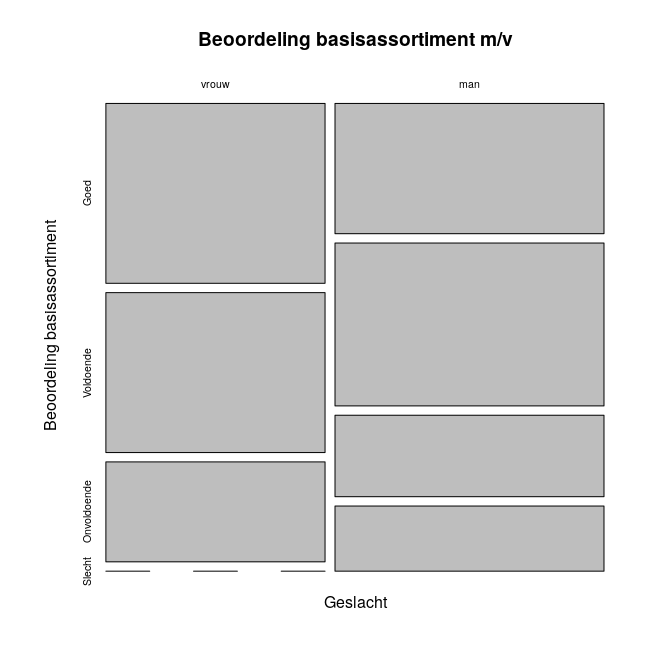
\includegraphics[height=.9\textheight]{img/2var-xtab-plot-waardering}
  \end{figure}
  
\end{frame}

\begin{frame}
  \frametitle{Visuele voorstelling van kruistabelen}
  \framesubtitle{Geclusterde staafgrafiek}

  \begin{figure}
    \centering
    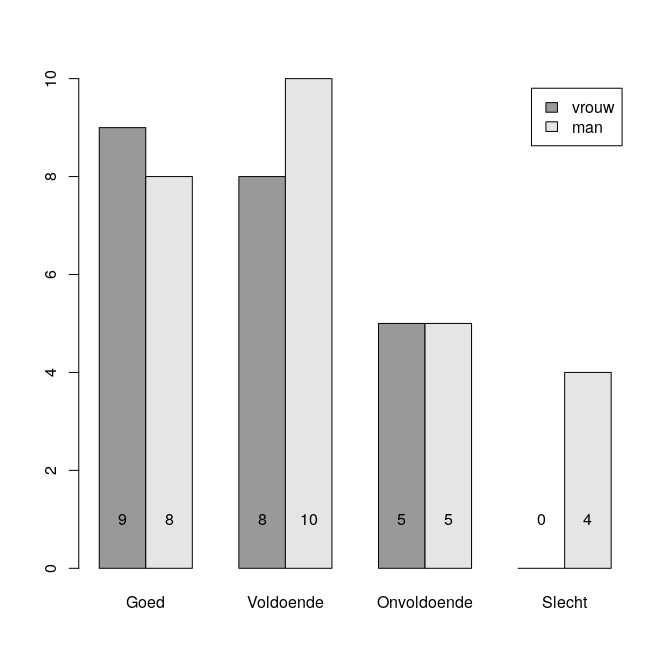
\includegraphics[height=.9\textheight]{img/2var-staafgrafiek-geclusterd}
  \end{figure}

\end{frame}

\begin{frame}
  \frametitle{Visuele voorstelling van kruistabelen}
  \framesubtitle{Rependiagram}
  
  \begin{figure}
    \centering
    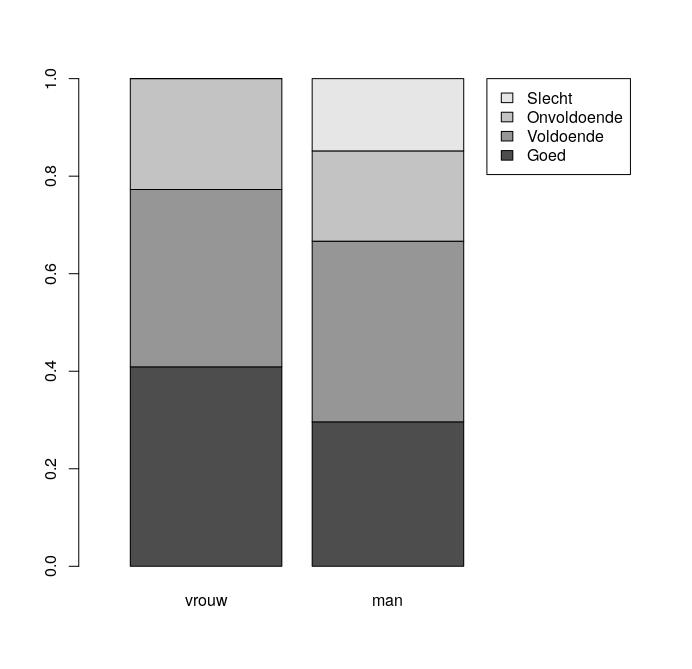
\includegraphics[height=.9\textheight]{img/2var-rependiagram-waardering-mv}
  \end{figure}

\end{frame}

\section{Lineaire Regressie}

\begin{frame}
  \frametitle{Lineaire regressie}
  \alertbox{Bij \textcolor{hgyellow}{regressie} gaan we proberen een \textcolor{hgyellow}{consistente} en \textcolor{hgyellow}{systematische} koppeling tussen de variabelen te vinden.}


  \begin{enumerate}
    \item \textbf{Monotoon:} algemene richting van de samenhang tussen de twee variabelen kan aangeduid worden (stijgend/dalend).
    \item \textbf{Niet-monotoon:}  aanwezigheid (of afwezigheid) van de ene variabele systematisch gerelateerd aan de aanwezigheid (of afwezigheid) van een andere variabele.
  \end{enumerate}
\end{frame}

\begin{frame}
  \frametitle{Lineaire regressie}
  Lineair verband: een rechtlijnige samenhang tussen een onafhankelijke en afhankelijke variabele, waarbij kennis van de onafhankelijke variabele kennis over de afhankelijke variabele geeft.
  \begin{itemize}
    \item Aanwezigheid
    \item Richting: dalend of stijgend?
    \item Sterke van het verband: sterk, gematigd, niet bestaand \dots
  \end{itemize}
\end{frame}

\begin{frame}
  \frametitle{Lineaire regressie}
  \centering
  \begin{tikzpicture}
    \begin{axis}[
        axis x line=middle,
        axis y line=middle,
        enlarge y limits=true,
        width=.9\textwidth, height=.9\textheight,     % size of the image
        grid = major,
        grid style={dashed, gray!30},
        ylabel=$y$,
        xlabel=$x$,
        legend style={at={(0.1,-0.1)}, anchor=north}
      ]
      \addplot[only marks] table  {data/regressie.dat};
    %\addplot [no markers, thick, red] table [y={create col/linear regression={y=y}}] {data/regressie.dat};
    \end{axis}
  \end{tikzpicture}
\end{frame}

\begin{frame}
  \frametitle{Lineaire regressie}
  \centering
  \begin{tikzpicture}
    \begin{axis}[
        axis x line=middle,
        axis y line=middle,
        enlarge y limits=true,
        width=.9\textwidth, height=.9\textheight,     % size of the image
        grid = major,
        grid style={dashed, gray!30},
        ylabel=$y$,
        xlabel=$x$,
        legend style={at={(0.1,-0.1)}, anchor=north}
      ]
      \addplot[only marks] table  {data/regressie.dat};
      \addplot [no markers, thick, red] table [y={create col/linear regression={y=y}}] {data/regressie.dat};
    \end{axis}
  \end{tikzpicture}
\end{frame}

\begin{frame}
  \frametitle{Kleinste kwadratenmethode: voorbeeld}
  \begin{columns}
    \begin{column}{0.5\textwidth}

      \begin{figure}
        \centering
        
\includegraphics[width=1.00\textwidth]{img/les3-santa.png}
        \label{fig:les3-santa}
      \end{figure}

    \end{column}
    \begin{column}{0.5\textwidth}

      \begin{figure}
        \centering
        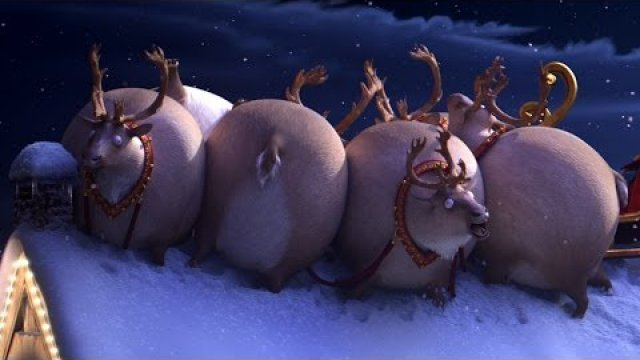
\includegraphics[width=1.00\textwidth]{img/les3-reindeer.jpg}
        \label{fig:les3-reindeer}
      \end{figure}

    \end{column}
  \end{columns}
  De Kerstman wil zijn rendieren vetmesten. Is er een verband
  tussen de hoeveelheid eiwitten in het dieet van de rendieren
  en hun gewichtstoename?

\end{frame}

\begin{frame}
  \frametitle{Kleinste kwadratenmethode: voorbeeld}
  \begin{table}[h]
    \centering
    \small
    \begin{tabular}{@{}rr@{}} \toprule
      Eiwitgehalte\%& Gewichtstoename (gram)  \\
      \midrule
      0   & 177 \\
      10  & 231 \\
      20  & 249 \\
      30  & 348 \\
      40  & 361 \\
      50  & 384 \\
      60  & 404 \\
      \bottomrule
    \end{tabular}
  \end{table}
\end{frame}

\begin{frame}
  \frametitle{Kleinste kwadratenmethode: voorbeeld}
  \centering
  \begin{tikzpicture}
    \begin{axis}[
        axis x line=middle,
        axis y line=middle,
        enlarge y limits=true,
        width=.9\textwidth, height=.9\textheight,     % size of the image
        grid = major,
        grid style={dashed, gray!30},
        ylabel=gewichtstoename (g),
        xlabel=eiwitgehalte (\%),
        legend style={at={(0.1,-0.1)}, anchor=north}
      ]
      \addplot[only marks] table  {data/santa.txt};
   % \addplot [no markers, thick, red] table [y={create col/linear regression={y=y}}] {data/santa.txt};
    \end{axis}
  \end{tikzpicture}
\end{frame}

\begin{frame}
  \frametitle{Kleinste kwadratenmethode: voorbeeld}
  \begin{table}[h] \centering \footnotesize
    \begin{tabular}{@{}llllll@{}}
      \toprule
      $x$   & $y$     & $x-\overline{x}$    & $y - \overline{y}$        & $(x-\overline{x})(y - \overline{y})$       &  $(x-\overline{x})^{2}$    \\ \midrule
      0  & 177 & -30 & -130,71 & 3921,3 & 900  \\
      10 & 231 & -20 & -76,71  & 1534,2 & 400  \\
      20 & 249 & -10 & -58,71  & 587,1  & 100  \\
      30 & 348 & 0   & 40,29   & 0      & 0    \\
      40 & 361 & 10  & 53,29   & 532,9  & 100  \\
      50 & 384 & 20  & 76,29   & 1525,8 & 400  \\
      60 & 404 & 30  & 96,29   & 2888,7 & 900  \\
      &     &     &         & 10990  & 2800 \\ \bottomrule
    \end{tabular}
    \caption{Berekeningen die nodig zijn voor het toepassen van de kleinste kwadratenmethode.}
    \label{tab:rendieren2}
  \end{table}
\end{frame}

\begin{frame}
\frametitle{Kleinste kwadratenmethode: formule}
  De regressierechte heeft als vergelijking:
  
  \[ y = \beta_1 x + \beta_0 \]
  
  met:
  
  \[ \beta_{1} = \frac{\sum_{i=1}^{n} (x_{i}-\overline{x})(y_{i} - \overline{y})}{\sum_{i=1}^{n} (x-\overline{x})^{2}} = \frac{10990}{2800} = 3.925 \]
  \[ \beta_{0} = \overline{y} - \beta_{1} \overline{x} = 307.7143 - 3.925 \times 30 = 189.96 \]
\end{frame}

\begin{frame}
  \frametitle{Kleinste kwadratenmethode: voorbeeld}
  \centering
  \begin{tikzpicture}
    \begin{axis}[
        axis x line=middle,
        axis y line=middle,
        enlarge y limits=true,
        width=.9\textwidth, height=.9\textheight,     % size of the image
        grid = major,
        grid style={dashed, gray!30},
        ylabel=gewichtstoename (g),
        xlabel=eiwitgehalte (\%),
        legend style={at={(0.1,-0.1)}, anchor=north}
      ]
      \addplot[only marks] table  {data/santa.txt};
      \addplot [no markers, thick, red] table [y={create col/linear regression={y=y}}] {data/santa.txt};
    \end{axis}
  \end{tikzpicture}
\end{frame}

\section{Correlatieco\"effici\"ent en determinatieco\"effci\"ent}

\begin{frame}
  \frametitle{Pearson correlatiecoëfficiënt en determinatiecoëfficiënt}
  \alertbox{De \textcolor{hgyellow}{Pearson correlatiecoëfficiënt} is een maat voor de sterkte van de lineaire samenhang tussen $x$ en $y$}

  \alertbox{De \textcolor{hgyellow}{determinatiecoëfficiënt} verklaart het percentage van de variantie van de waargenomen waarden t.o.v. de regressierechte.}
\end{frame}

\begin{frame}
  \frametitle{Covariantie}
  We plotten de gezinsgrootte van 15 families tot de gezinsgrootte van de moeder toen ze klein was.

  \centering
  \begin{tikzpicture}
    \begin{axis}[
        axis x line=middle,
        axis y line=middle,
        enlarge y limits=true,
        width=.9\textwidth, height=.9\textheight,     % size of the image
        grid = major,
        grid style={dashed, gray!30},
        ylabel=gezinsgrootte moeder,
        xlabel=gezinsgrootte,
        legend style={at={(0.1,-0.1)}, anchor=north}
      ]
      \addplot[only marks] table  {data/families.txt};
      \addplot [no markers, thick, red] table [y={create col/linear regression={y=y}}] {data/families.txt};
    \end{axis}
  \end{tikzpicture}
  We vinden $\overline{x} = 3$ en $\overline{y} = 4.3$.
\end{frame}

\tikzset{small dot/.style={fill=black, circle,scale=0.2}}
\tikzset{every pin/.style={draw=black,fill=yellow!10}}

\begin{frame}
  \frametitle{Covariantie bij lineair verband}
  \centering
  \begin{tikzpicture}
    \begin{axis}[
        axis x line=middle,
        axis y line=middle,
        enlarge y limits=true,
        width=.9\textwidth, height=.9\textheight,     % size of the image
        grid = major,
        grid style={dashed, gray!30},
        ylabel=gezinsgrootte moeder,
        xlabel=gezinsgrootte,
        legend style={at={(0.1,-0.1)}, anchor=north}
      ]
      \draw (axis cs:3,0)--(axis cs:3,8);
      \draw (axis cs:0,4.3)--(axis cs:6,4.3);
      \node[small dot, pin=120:{$III$}] at (axis cs:1.9,6) {};
      \node[small dot, pin=120:{$I$}] at (axis cs:4.5,6) {};
      \node[small dot, pin=120:{$II$}] at (axis cs:1.9,2) {};
      \node[small dot, pin=120:{$IV$}] at (axis cs:4.5,2) {};
      \addplot[only marks] table  {data/families.txt};
    \end{axis}
  \end{tikzpicture}
\end{frame}

\begin{frame}
  \frametitle{Covariantie bij willekeurigheid}
  \centering
  \begin{tikzpicture}
    \begin{axis}[
        axis x line=middle,
        axis y line=middle,
        enlarge y limits=true,
        width=.9\textwidth, height=.9\textheight,     % size of the image
        grid = major,
        grid style={dashed, gray!30},
        ylabel=gezinsgrootte moeder,
        xlabel=geboortedatum moeder,
        legend style={at={(0.1,-0.1)}, anchor=north}
      ]
      \draw (axis cs:1942.625,0)--(axis cs:1942.625,6);
      \draw (axis cs:1930,3.4375)--(axis cs:1955,3.4375);
      \node[small dot, pin=120:{$III$}] at (axis cs:1935,5) {};
      \node[small dot, pin=120:{$I$}] at (axis cs:1950,5) {};
      \node[small dot, pin=120:{$II$}] at (axis cs:1935,2) {};
      \node[small dot, pin=120:{$IV$}] at (axis cs:1950,2) {};
      \addplot[only marks] table  {data/families2.txt};
    \end{axis}
  \end{tikzpicture}
  We vinden $\overline{x} = 1942.625$ en $\overline{y} = 3.4375$.
\end{frame}


\begin{frame}
  \frametitle{Determinatieco\"effici\"ent}
  \begin{figure}[t]
    \begin{tikzpicture}
      \begin{axis}[
          axis x line=middle,
          axis y line=middle,
          enlarge y limits=true,
          width=.9\textwidth, height=.9\textheight,     % size of the image
          grid = major,
          grid style={dashed, gray!30},
          ylabel=gewichtstoename (g),
          xlabel=eiwitgehalte (\%),
          legend style={at={(0.1,-0.1)}, anchor=north}
        ]
        \addplot[only marks] table  {data/santa.txt};
        \addplot [no markers, thick, red] table [y={create col/linear regression={y=y}}] {data/santa.txt};
        \addplot [mark=none, color=red] coordinates {
          (0,177) (0,189.9643)
        };
        \addplot [mark=none, color=red] coordinates {
          (10,231) (10,229.2143)
        };
        \addplot [mark=none, color=red] coordinates {
          (20,249) (20,268.4643)
        };
        \addplot [mark=none, color=red] coordinates {
          (30,348) (30,307.7143)
        };
        \addplot [mark=none, color=red] coordinates {
          (40,361) (40,346.9643)
        };
        \addplot [mark=none, color=red] coordinates {
          (50,384) (50,386.2143)
        };
        \addplot [mark=none, color=red] coordinates {
          (60,404) (60,425.4643)
        };

      \end{axis}
    \end{tikzpicture}
    \label{fig:rendierenFiguur2}
    \caption{Deviaties tot de regressierechte: aanname $x$ geeft extra informatie voor het voorspellen van $y$.}
  \end{figure}
\end{frame}

\begin{frame}
  \begin{figure}[t]
    \begin{tikzpicture}
      \begin{axis}[
          axis x line=middle,
          axis y line=middle,
          enlarge y limits=true,
          width=.9\textwidth, height=.9\textheight,     % size of the image
          grid = major,
          grid style={dashed, gray!30},
          ylabel=gewichtstoename (g),
          xlabel=eiwitgehalte (\%),
        ]
        \addplot[only marks] table  {data/santa.txt};
        \addplot [mark=none, color=black] coordinates {
          (0,307.71) (60,307.71)
        };
        \addplot [mark=none, color=red] coordinates {
          (0,177) (0,307.71)
        };
        \addplot [mark=none, color=red] coordinates {
          (10,231) (10,307.71)
        };
        \addplot [mark=none, color=red] coordinates {
          (20,249) (20,307.71)
        };
        \addplot [mark=none, color=red] coordinates {
          (30,348) (30,307.71)
        };
        \addplot [mark=none, color=red] coordinates {
          (40,361) (40,307.71)
        };
        \addplot [mark=none, color=red] coordinates {
          (50,384) (50,307.71)
        };
        \addplot [mark=none, color=red] coordinates {
          (60,404) (60,307.71)
        };

      \end{axis}
    \end{tikzpicture}
    \label{fig:rendierenFiguur3}
    \caption{Deviaties tot de gemiddelde van y: aanname $x$ geeft geen informatie voor het voorspellen van $y$ ($\overline{y} =307.71$).}
  \end{figure}
\end{frame}

\begin{frame}
  \frametitle{Correlatieco\"effici\"ent en determinatieco\"effci\"ent}
  \begin{table}[h] \centering \small
    \begin{tabular}{@{}|r|r|r|r|@{}} \toprule
      $R$ & $R^{2}$ & Verklaarde variantie &  Interpretatie \\
      \midrule
      $< 0,3$       & $< 0,1$       & $< 10\%$    & zeer zwak \\
      $0,3 - 0,5$   & $0,1 - 0,25r$ & $10 - 25\%$ & zwak \\
      $0,5 - 0,7$   & $0,25 - 0,5$  & $25 - 50\%$ & matig\\
      $0,7 - 0,85$  & $0,5 - 0,75$  & $50 - 75\%$ & sterk\\
      $0,85 - 0,95$ & $0,75 - 0,9$  & $75 - 90\%$ & zeer sterk\\
      $> 0,95$      & $> 0,9$       & $>90\%$     & uitzonderlijk(!)\\
      \bottomrule
    \end{tabular}
  \end{table}

\end{frame}

\begin{frame}
  \frametitle{Sterkte verband rendieren}
  \begin{columns}
    \begin{column}{0.5\textwidth}
      \begin{table}[h] \centering \small
        \begin{tabular}{@{}rrr@{}} \toprule
          $(x-\overline{x})$ & $(y - \overline{y})$ & $(x-\overline{x})(y - \overline{y})$ \\
          \midrule
          $-30$ & $-130.714$ & $3921.429$ \\
          $-20$ & $-76.7143$ & $1534.286$ \\
          $-10$ & $-58.7143$ & $587.1429$\\
          $0$   & $40.28571$ & $0$\\
          $10$  & $53.28571$ & $532.8571$\\
          $20$  & $76.28571$ & $1525.714$\\
          $30$  & $96.28571$ & $2888.571$\\
          \bottomrule
        \end{tabular}
      \end{table}
    \end{column}
    \begin{column}{0.5\textwidth}
      \[ \sum_{i}^{n} (x-\overline{x})(y - \overline{y}) = 10990 \]
      \[ Cov = \frac{10990}{7} = 1570 \]
      \[ \sigma_{x} = 20 \]
      \[ \sigma_{y} = 81.03 \]
      \[ R = \frac{1570}{20 \times 81.03} = 0.96 \]
      \[ R^{2} = 0.93 \]
    \end{column}
  \end{columns}
\end{frame}

\begin{frame}
  \frametitle{Overwegingen}
  \begin{itemize}
    \item Bij de correlatiecoëfficiënt wordt er alleen naar het verband tussen twee variabelen gekeken. Er wordt niet gekeken naar interacties met andere variabelen.
    \item Er wordt bij de correlatiecoëfficiënt expliciet niet uitgegaan van een oorzaak-en gevolg verband
    \item De product-momentcorrelatiecoëfficiënt van Pearson drukt slechts lineaire verbanden uit
  \end{itemize}
\end{frame}

\begin{frame}
  \frametitle{Verband regressierechte en correlateco\"effici\"ent}

  \begin{figure}
    \centering
    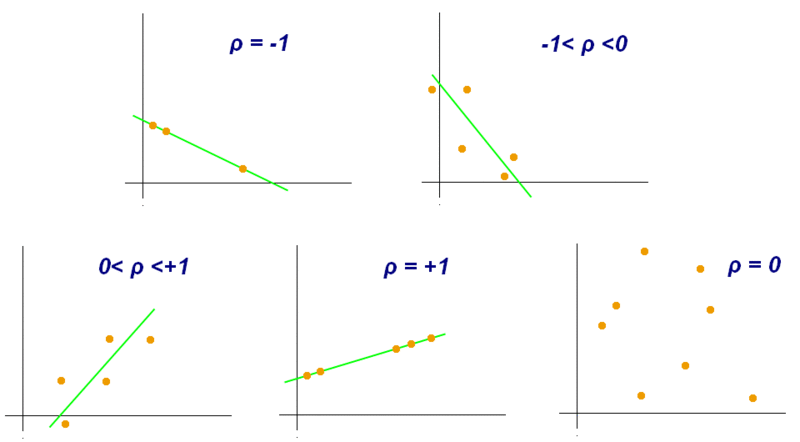
\includegraphics[height=\textheight]{img/les3-regressie.png}
    \label{fig:les3-regressie}
  \end{figure}

\end{frame}

%---------- Back matter -------------------------------------------------------

\end{document}
